
%% This template is an adaption from the original IEEE conference class
%% (bare_conf.tex  V1.4a) by Michael Shell.

%%*************************************************************************
%% Comments from the original author:
%% bare_conf.tex
%% V1.4a
%% 2014/09/17
%% by Michael Shell
%% See:
%% http://www.michaelshell.org/
%% for current contact information.
%%
%% This is a skeleton file demonstrating the use of IEEEtran.cls
%% (requires IEEEtran.cls version 1.8a or later) with an IEEE
%% conference paper.
%%
%% Support sites:
%% http://www.michaelshell.org/tex/ieeetran/
%% http://www.ctan.org/tex-archive/macros/latex/contrib/IEEEtran/
%% and
%% http://www.ieee.org/

%%*************************************************************************
%% Legal Notice:
%% This code is offered as-is without any warranty either expressed or
%% implied; without even the implied warranty of MERCHANTABILITY or
%% FITNESS FOR A PARTICULAR PURPOSE! 
%% User assumes all risk.
%% In no event shall IEEE or any contributor to this code be liable for
%% any damages or losses, including, but not limited to, incidental,
%% consequential, or any other damages, resulting from the use or misuse
%% of any information contained here.
%%
%% All comments are the opinions of their respective authors and are not
%% necessarily endorsed by the IEEE.
%%
%% This work is distributed under the LaTeX Project Public License (LPPL)
%% ( http://www.latex-project.org/ ) version 1.3, and may be freely used,
%% distributed and modified. A copy of the LPPL, version 1.3, is included
%% in the base LaTeX documentation of all distributions of LaTeX released
%% 2003/12/01 or later.
%% Retain all contribution notices and credits.
%% ** Modified files should be clearly indicated as such, including  **
%% ** renaming them and changing author support contact information. **
%%
%% File list of work: IEEEtran.cls, IEEEtran_HOWTO.pdf, bare_adv.tex,
%%                    bare_conf.tex, bare_jrnl.tex, bare_conf_compsoc.tex,
%%                    bare_jrnl_compsoc.tex, bare_jrnl_transmag.tex
%%*************************************************************************


% *** Authors should verify (and, if needed, correct) their LaTeX system  ***
% *** with the testflow diagnostic prior to trusting their LaTeX platform ***
% *** with production work. IEEE's font choices and paper sizes can       ***
% *** trigger bugs that do not appear when using other class files.       ***                          ***
% The testflow support page is at:
% http://www.michaelshell.org/tex/testflow/



% \documentclass[a4paper,oneside,onecolumn,draft,12pt,conference]{IEEEtran}
\documentclass[a4paper,oneside,onecolumn,draftcls,12pt,conference]{IEEEtran}
%\documentclass[a4paper,oneside,onecolumn,draftclsnofoot,12pt,conference]{IEEEtran} 
%\documentclass[letterpaper,oneside,onecolumn,draftclsnofoot,12pt,conference]{IEEEtran}  
 
 
 
 
% Some very useful LaTeX packages include:
% (uncomment the ones you want to load)


% *** MISC UTILITY PACKAGES ***
%
%\usepackage{ifpdf}
% Heiko Oberdiek's ifpdf.sty is very useful if you need conditional
% compilation based on whether the output is pdf or dvi.
% usage:
% \ifpdf
%   % pdf code
% \else
%   % dvi code
% \fi
% The latest version of ifpdf.sty can be obtained from:
% http://www.ctan.org/tex-archive/macros/latex/contrib/oberdiek/
% Also, note that IEEEtran.cls V1.7 and later provides a builtin
% \ifCLASSINFOpdf conditional that works the same way.
% When switching from latex to pdflatex and vice-versa, the compiler may
% have to be run twice to clear warning/error messages.

%\usepackage{IEEEtrantools}


% *** CITATION PACKAGES ***
%
\usepackage{cite}
% cite.sty was written by Donald Arseneau
% V1.6 and later of IEEEtran pre-defines the format of the cite.sty package
% \cite{} output to follow that of IEEE. Loading the cite package will
% result in citation numbers being automatically sorted and properly
% "compressed/ranged". e.g., [1], [9], [2], [7], [5], [6] without using
% cite.sty will become [1], [2], [5]--[7], [9] using cite.sty. cite.sty's
% \cite will automatically add leading space, if needed. Use cite.sty's
% noadjust option (cite.sty V3.8 and later) if you want to turn this off
% such as if a citation ever needs to be enclosed in parenthesis.
% cite.sty is already installed on most LaTeX systems. Be sure and use
% version 5.0 (2009-03-20) and later if using hyperref.sty.
% The latest version can be obtained at:
% http://www.ctan.org/tex-archive/macros/latex/contrib/cite/
% The documentation is contained in the cite.sty file itself.






% *** GRAPHICS RELATED PACKAGES ***
%
\ifCLASSINFOpdf
   \usepackage[pdftex]{graphicx}
  % declare the path(s) where your graphic files are
  % \graphicspath{{../pdf/}{../jpeg/}}
  % and their extensions so you won't have to specify these with
  % every instance of \includegraphics
  % \DeclareGraphicsExtensions{.pdf,.jpeg,.png}
\else
  % or other class option (dvipsone, dvipdf, if not using dvips). graphicx
  % will default to the driver specified in the system graphics.cfg if no
  % driver is specified.
  % \usepackage[dvips]{graphicx}
  % declare the path(s) where your graphic files are
  % \graphicspath{{../eps/}}
  % and their extensions so you won't have to specify these with
  % every instance of \includegraphics
  % \DeclareGraphicsExtensions{.eps}
\fi
% graphicx was written by David Carlisle and Sebastian Rahtz. It is
% required if you want graphics, photos, etc. graphicx.sty is already
% installed on most LaTeX systems. The latest version and documentation
% can be obtained at: 
% http://www.ctan.org/tex-archive/macros/latex/required/graphics/
% Another good source of documentation is "Using Imported Graphics in
% LaTeX2e" by Keith Reckdahl which can be found at:
% http://www.ctan.org/tex-archive/info/epslatex/
%
% latex, and pdflatex in dvi mode, support graphics in encapsulated
% postscript (.eps) format. pdflatex in pdf mode supports graphics
% in .pdf, .jpeg, .png and .mps (metapost) formats. Users should ensure
% that all non-photo figures use a vector format (.eps, .pdf, .mps) and
% not a bitmapped formats (.jpeg, .png). IEEE frowns on bitmapped formats
% which can result in "jaggedy"/blurry rendering of lines and letters as
% well as large increases in file sizes.
%
% You can find documentation about the pdfTeX application at:
% http://www.tug.org/applications/pdftex





% *** MATH PACKAGES ***
%
\usepackage[cmex10]{amsmath}
% A popular package from the American Mathematical Society that provides
% many useful and powerful commands for dealing with mathematics. If using
% it, be sure to load this package with the cmex10 option to ensure that
% only type 1 fonts will utilized at all point sizes. Without this option,
% it is possible that some math symbols, particularly those within
% footnotes, will be rendered in bitmap form which will result in a
% document that can not be IEEE Xplore compliant!
%
% Also, note that the amsmath package sets \interdisplaylinepenalty to 10000
% thus preventing page breaks from occurring within multiline equations. Use:
%\interdisplaylinepenalty=2500
% after loading amsmath to restore such page breaks as IEEEtran.cls normally
% does. amsmath.sty is already installed on most LaTeX systems. The latest
% version and documentation can be obtained at:
% http://www.ctan.org/tex-archive/macros/latex/required/amslatex/math/





% *** SPECIALIZED LIST PACKAGES ***
%
\usepackage{algorithmic}
% algorithmic.sty was written by Peter Williams and Rogerio Brito.
% This package provides an algorithmic environment fo describing algorithms.
% You can use the algorithmic environment in-text or within a figure
% environment to provide for a floating algorithm. Do NOT use the algorithm
% floating environment provided by algorithm.sty (by the same authors) or
% algorithm2e.sty (by Christophe Fiorio) as IEEE does not use dedicated
% algorithm float types and packages that provide these will not provide
% correct IEEE style captions. The latest version and documentation of
% algorithmic.sty can be obtained at:
% http://www.ctan.org/tex-archive/macros/latex/contrib/algorithms/
% There is also a support site at:
% http://algorithms.berlios.de/index.html
% Also of interest may be the (relatively newer and more customizable)
% algorithmicx.sty package by Szasz Janos:
% http://www.ctan.org/tex-archive/macros/latex/contrib/algorithmicx/




% *** ALIGNMENT PACKAGES ***
%
\usepackage{array}
% Frank Mittelbach's and David Carlisle's array.sty patches and improves
% the standard LaTeX2e array and tabular environments to provide better
% appearance and additional user controls. As the default LaTeX2e table
% generation code is lacking to the point of almost being broken with
% respect to the quality of the end results, all users are strongly
% advised to use an enhanced (at the very least that provided by array.sty)
% set of table tools. array.sty is already installed on most systems. The
% latest version and documentation can be obtained at:
% http://www.ctan.org/tex-archive/macros/latex/required/tools/


% IEEEtran contains the IEEEeqnarray family of commands that can be used to
% generate multiline equations as well as matrices, tables, etc., of high
% quality.




% *** SUBFIGURE PACKAGES ***
\ifCLASSOPTIONcompsoc
  \usepackage[caption=false,font=normalsize,labelfont=sf,textfont=sf]{subfig}
\else
  \usepackage[caption=false,font=footnotesize]{subfig}
\fi
% subfig.sty, written by Steven Douglas Cochran, is the modern replacement
% for subfigure.sty, the latter of which is no longer maintained and is
% incompatible with some LaTeX packages including fixltx2e. However,
% subfig.sty requires and automatically loads Axel Sommerfeldt's caption.sty
% which will override IEEEtran.cls' handling of captions and this will result
% in non-IEEE style figure/table captions. To prevent this problem, be sure
% and invoke subfig.sty's "caption=false" package option (available since
% subfig.sty version 1.3, 2005/06/28) as this is will preserve IEEEtran.cls
% handling of captions.
% Note that the Computer Society format requires a larger sans serif font
% than the serif footnote size font used in traditional IEEE formatting
% and thus the need to invoke different subfig.sty package options depending
% on whether compsoc mode has been enabled.
%
% The latest version and documentation of subfig.sty can be obtained at:
% http://www.ctan.org/tex-archive/macros/latex/contrib/subfig/




% *** FLOAT PACKAGES ***
%
%\usepackage{fixltx2e}
% fixltx2e, the successor to the earlier fix2col.sty, was written by
% Frank Mittelbach and David Carlisle. This package corrects a few problems
% in the LaTeX2e kernel, the most notable of which is that in current
% LaTeX2e releases, the ordering of single and double column floats is not
% guaranteed to be preserved. Thus, an unpatched LaTeX2e can allow a
% single column figure to be placed prior to an earlier double column
% figure. The latest version and documentation can be found at:
% http://www.ctan.org/tex-archive/macros/latex/base/


%\usepackage{stfloats}
% stfloats.sty was written by Sigitas Tolusis. This package gives LaTeX2e
% the ability to do double column floats at the bottom of the page as well
% as the top. (e.g., "\begin{figure*}[!b]" is not normally possible in
% LaTeX2e). It also provides a command:
%\fnbelowfloat
% to enable the placement of footnotes below bottom floats (the standard
% LaTeX2e kernel puts them above bottom floats). This is an invasive package
% which rewrites many portions of the LaTeX2e float routines. It may not work
% with other packages that modify the LaTeX2e float routines. The latest
% version and documentation can be obtained at:
% http://www.ctan.org/tex-archive/macros/latex/contrib/sttools/
% Do not use the stfloats baselinefloat ability as IEEE does not allow
% \baselineskip to stretch. Authors submitting work to the IEEE should note
% that IEEE rarely uses double column equations and that authors should try
% to avoid such use. Do not be tempted to use the cuted.sty or midfloat.sty
% packages (also by Sigitas Tolusis) as IEEE does not format its papers in
% such ways.
% Do not attempt to use stfloats with fixltx2e as they are incompatible.
% Instead, use Morten Hogholm'a dblfloatfix which combines the features
% of both fixltx2e and stfloats:
%
% \usepackage{dblfloatfix}
% The latest version can be found at:
% http://www.ctan.org/tex-archive/macros/latex/contrib/dblfloatfix/




% *** PDF, URL AND HYPERLINK PACKAGES ***
%
\usepackage{url}
% url.sty was written by Donald Arseneau. It provides better support for
% handling and breaking URLs. url.sty is already installed on most LaTeX
% systems. The latest version and documentation can be obtained at:
% http://www.ctan.org/tex-archive/macros/latex/contrib/url/
% Basically, \url{my_url_here}.


% *** Do not adjust lengths that control margins, column widths, etc. ***
% *** Do not use packages that alter fonts (such as pslatex).         ***
% There should be no need to do such things with IEEEtran.cls V1.6 and later.
% (Unless specifically asked to do so by the journal or conference you plan
% to submit to, of course. )


% *** YOU STILL MAY ADD NEW PACKAGES ***
% Be careful including new packages that can handle with caption
% or change the default layout.

\usepackage{float}
\usepackage{booktabs}

\usepackage[utf8]{inputenc}	 % Document Encoding (automatic conversion of accents)
\usepackage{cite}      % Written by Donald Arseneau         
\usepackage{epstopdf}

\usepackage{datetime}

\usepackage{siunitx}
\sisetup{detect-all}
\sisetup{round-mode=places,round-precision=2}
\DeclareSIUnit \VA {VA} %apparent power

\usepackage{wrapfig} % Al­lows fig­ures or ta­bles to have text wrapped around them


% correct bad hyphenation here
\hyphenation{op-tical net-works semi-conduc-tor}


\begin{document}
%
% paper title
% Titles are generally capitalized except for words such as a, an, and, as,
% at, but, by, for, in, nor, of, on, or, the, to and up, which are usually
% not capitalized unless they are the first or last word of the title.
% Linebreaks \\ can be used within to get better formatting as desired.
% Do not put math or special symbols in the title.
\title{Digest Demo of IEEEtran.cls \cite{IEEEhowto:IEEEtranpage} for COBEP 2015}


% author names and affiliations
% use a multiple column layout for up to three different
% affiliations
%\author{\IEEEauthorblockN{Michael Shell}
%\IEEEauthorblockA{School of Electrical and\\Computer Engineering\\
%Georgia Institute of Technology\\
%Atlanta, Georgia 30332--0250\\
%Email: http://www.michaelshell.org/contact.html}
%\and
%\IEEEauthorblockN{Homer Simpson}
%\IEEEauthorblockA{Twentieth Century Fox\\
%Springfield, USA\\
%Email: homer@thesimpsons.com}
%\and
%\IEEEauthorblockN{James Kirk\\ and Montgomery Scott}
%\IEEEauthorblockA{Starfleet Academy\\
%San Francisco, California 96678--2391\\
%Telephone: (800) 555--1212\\
%Fax: (888) 555--1212}}

% conference papers do not typically use \thanks and this command
% is locked out in conference mode. If really needed, such as for
% the acknowledgment of grants, issue a \IEEEoverridecommandlockouts
% after \documentclass

% for over three affiliations, or if they all won't fit within the width
% of the page, use this alternative format:
% 
%\author{\IEEEauthorblockN{Michael Shell\IEEEauthorrefmark{1},
%Homer Simpson\IEEEauthorrefmark{2},
%James Kirk\IEEEauthorrefmark{3}, 
%Montgomery Scott\IEEEauthorrefmark{3} and
%Eldon Tyrell\IEEEauthorrefmark{4}}
%\IEEEauthorblockA{\IEEEauthorrefmark{1}School of Electrical and Computer Engineering\\
%Georgia Institute of Technology,
%Atlanta, Georgia 30332--0250\\ Email: see http://www.michaelshell.org/contact.html}
%\IEEEauthorblockA{\IEEEauthorrefmark{2}Twentieth Century Fox, Springfield, USA\\
%Email: homer@thesimpsons.com}
%\IEEEauthorblockA{\IEEEauthorrefmark{3}Starfleet Academy, San Francisco, California 96678-2391\\
%Telephone: (800) 555--1212, Fax: (888) 555--1212}
%\IEEEauthorblockA{\IEEEauthorrefmark{4}Tyrell Inc., 123 Replicant Street, Los Angeles, California 90210--4321}}


% make the title area
\maketitle

% As a general rule, do not put math, special symbols or citations
% in the abstract
\begin{abstract}
The Brazilian Power Electronics Conference -- COBEP is a conference held every odd year in Brazil, since 1991, supported by the Brazilian Power Electronics Society -- SOBRAEP. Due to high technical and scientific levels COBEP has long been technically sponsored by the IEEE. For 2015 we are pleased to introduce the first IEEE Southern Power Electronic Conference -- SPEC along with COBEP in a unique event of power electronics in the Southern hemisphere.
\end{abstract}

% no keywords

%\begin{IEEEkeywords}
%	Broad band networks, quality of service, WDM.
%\end{IEEEkeywords}



% For peer review papers, you can put extra information on the cover
% page as needed:
% \ifCLASSOPTIONpeerreview
% \begin{center} \bfseries EDICS Category: 3-BBND \end{center}
% \fi
%
% For peerreview papers, this IEEEtran command inserts a page break and
% creates the second title. It will be ignored for other modes.
\IEEEpeerreviewmaketitle



\section{Introduction}
% no \IEEEPARstart

The conference covers the fields of interest of the power electronics community, providing a forum for sharing theoretical and practical developments related to power electronics, featuring strong participation of industry and academia.
The main topics of the conference include.


\begin{enumerate}
\item	Power converters topologies and design;
\item	Electrical machines and drive systems;
\item	Modeling, simulation and control in power electronics;
\item	Devices,   packaging,   integration,   magnetic   materials   and passive components;
\item	Industrial, commercial and residential applications;
\item	Renewable energy systems;
\item	Smart grid and utility applications;
\item	Energy  efficiency,   power   quality   and   electromagnetic compatibility;
\item	Education and special topics.	
\end{enumerate}



\section{The Venue}




Fortaleza is a seaside town in the Northeast of Brazil, in Ceará State, with 300 days of sunshine per year, an average annual temperature around \SI{27}{\degreeCelsius} (\SI{80}{\degree F}) and beaches with warm water. A constant and pleasant wind makes the place ideal for sports like windsurf and surf, as well as to produce electricity from wind parks. Fortaleza has many attractions that you can discover them just being there.



\subsubsection{The conference will be held at}
Ponta Mar Hotel (\url{http://www.praiacentro.com.br}) 740 Av. Monsenhor Tabosa -- Fortaleza -- CE -- Brazil

\section{Paper Submission Guideline and Format}


\begin{wraptable}{R}{0.45\textwidth}
	\vspace{-20pt}
	\begin{center}
		\caption{A wrapped table going nicely inside the text.}\label{wrap-tab:1}
		\begin{tabular}{ccc}\\\toprule  
			Header-1 & Header-1 & Header-1 \\\midrule
			2 &3 & 5\\  \midrule
			2 &3 & 5\\  \midrule
			2 &3 & 5\\  \bottomrule
		\end{tabular}
	\end{center}
	\vspace{-20pt}
	\vspace{1pt}
\end{wraptable} 

Prospective authors are requested to submit a digest no longer than five (5) pages, single column, double spaced, font size 12, summarizing the proposed paper. The digest should include key equations, figures, tables and references as appropriate, but no author names or affiliations. The digests must clearly state the objectives of the work, its significance in advancing engineering or science, and the methods and specific results in sufficient detail. Papers presented at COBEP/SPEC must be original material and not have been previously presented or published. Reviewers value evidence of completed experimental work. Authors should obtain any necessary company and governmental clearance prior to submission of digests.



\begin{wrapfigure}{R}{0.45\textwidth} 
	\vspace{-20pt}
	\begin{center}
	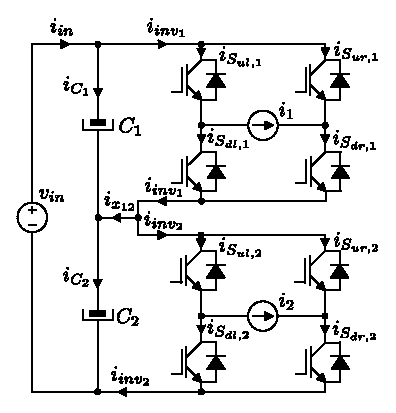
\includegraphics[width=0.4\textwidth]{Figs/MHF1F_ix.eps}
	\caption{Equivalent circuit used to analyze the capacitor voltage for two sub-modules.}
	\label{fig:MHF1F_ix3}
	\end{center}
	\vspace{-20pt}
	\vspace{1pt}
\end{wrapfigure} 


Contributing authors may submit digest written in English following all details on digest and final manuscript format available on-line at \url{www.cobepspec2015.ufc.br}.



If a digest is accepted, authors must submit a final manuscript before the deadline or the manuscript cannot be published in the Proceedings or presented at the conference. Final manuscripts may be subject to charges if their papers are over the page or file size limit. At least one of the authors listed on a paper must be registered for either a Full Registration or for the Technical Sessions Only registration, per paper.




% An example of a floating figure using the graphicx package.
% Note that \label must occur AFTER (or within) \caption.
% For figures, \caption should occur after the \includegraphics.
% Note that IEEEtran v1.7 and later has special internal code that
% is designed to preserve the operation of \label within \caption
% even when the captionsoff option is in effect. However, because
% of issues like this, it may be the safest practice to put all your
% \label just after \caption rather than within \caption{}.
%
% Reminder: the "draftcls" or "draftclsnofoot", not "draft", class
% option should be used if it is desired that the figures are to be
% displayed while in draft mode.
%
%\begin{figure}[!t]
%\centering
%\includegraphics[width=2.5in]{myfigure}
% where an .eps filename suffix will be assumed under latex, 
% and a .pdf suffix will be assumed for pdflatex; or what has been declared
% via \DeclareGraphicsExtensions.
%\caption{Simulation results for the network.}
%\label{fig_sim}
%\end{figure}

% Note that IEEE typically puts floats only at the top, even when this
% results in a large percentage of a column being occupied by floats.


% An example of a double column floating figure using two subfigures.
% (The subfig.sty package must be loaded for this to work.)
% The subfigure \label commands are set within each subfloat command,
% and the \label for the overall figure must come after \caption.
% \hfil is used as a separator to get equal spacing.
% Watch out that the combined width of all the subfigures on a 
% line do not exceed the text width or a line break will occur.
%
%\begin{figure*}[!t]
%\centering
%\subfloat[Case I]{\includegraphics[width=2.5in]{box}%
%\label{fig_first_case}}
%\hfil
%\subfloat[Case II]{\includegraphics[width=2.5in]{box}%
%\label{fig_second_case}}
%\caption{Simulation results for the network.}
%\label{fig_sim}
%\end{figure*}
%
% Note that often IEEE papers with subfigures do not employ subfigure
% captions (using the optional argument to \subfloat[]), but instead will
% reference/describe all of them (a), (b), etc., within the main caption.
% Be aware that for subfig.sty to generate the (a), (b), etc., subfigure
% labels, the optional argument to \subfloat must be present. If a
% subcaption is not desired, just leave its contents blank,
% e.g., \subfloat[].


% An example of a floating table. Note that, for IEEE style tables, the
% \caption command should come BEFORE the table and, given that table
% captions serve much like titles, are usually capitalized except for words
% such as a, an, and, as, at, but, by, for, in, nor, of, on, or, the, to
% and up, which are usually not capitalized unless they are the first or
% last word of the caption. Table text will default to \footnotesize as
% IEEE normally uses this smaller font for tables.
% The \label must come after \caption as always.
%
%\begin{table}[!t]
%% increase table row spacing, adjust to taste
%\renewcommand{\arraystretch}{1.3}
% if using array.sty, it might be a good idea to tweak the value of
% \extrarowheight as needed to properly center the text within the cells
%\caption{An Example of a Table}
%\label{table_example}
%\centering
%% Some packages, such as MDW tools, offer better commands for making tables
%% than the plain LaTeX2e tabular which is used here.
%\begin{tabular}{|c||c|}
%\hline
%One & Two\\
%\hline
%Three & Four\\
%\hline
%\end{tabular}
%\end{table}


% Note that the IEEE does not put floats in the very first column
% - or typically anywhere on the first page for that matter. Also,
% in-text middle ("here") positioning is typically not used, but it
% is allowed and encouraged for Computer Society conferences (but
% not Computer Society journals). Most IEEE journals/conferences use
% top floats exclusively. 
% Note that, LaTeX2e, unlike IEEE journals/conferences, places
% footnotes above bottom floats. This can be corrected via the
% \fnbelowfloat command of the stfloats package.




\section{Important dates }

PAPER SUBMISSION: MARCH 30th to MAY 1st

Notification of Acceptance:     Jul. 29, 2015 Final Version:	Aug. 28, 2015



% conference papers do not normally have an appendix


% use section* for acknowledgment
%\section*{Acknowledgment}

\section*{Local Committee}


Prof. Fernando Luiz Marcelo Antunes, (General Chair)  
 
Prof. Luiz Henrique Silva Colado Barreto (General co--Chair) 

Prof. Demercil de Sousa Oliveira Junior, (Programme Chair)

Prof. Paulo Peixoto Praça (Treasurer)





\section{Some Latex Test}

 
 \subsection{Equations}
 \begin{equation}
 \Delta I_{L}=I_{o}+\frac{\sqrt{3}}{2}.\frac{V_{i}}{Z}
 \end{equation}
 Where:
 
 \begin{enumerate}
 	\item[$\Delta I_{L}$]  - Peak value of resonant current.
 	\item[$I_{o}$]  - Load current.
 	\item[$V_{i}$]  - Input voltage.
 	\item[$Z$]  - Characteristic impedance of the resonant circuit.
 \end{enumerate}
 
  \begin{equation} \label{eq:ix12}
  {i_{{x_{12}}}}\left( \theta  \right) = \frac{{{m_o}}}{2}\left[ {{I_1}\cos \left( {{\theta _1}} \right) - {I_2}\cos \left( {{\theta _2}} \right)} \right]
  + \frac{{{m_o}{I_2}}}{2}\cos \left( {2\theta  + {\theta _2}} \right) - \frac{{{m_o}{I_1}}}{2}\cos \left( {2\theta  + {\theta _1}} \right).	
  \end{equation}
  
  	\begin{eqnarray}
  		{v_{ds}} &=& {R_s}{i_{ds}} + \frac{{d{\psi _{ds}}}}{{dt}} - {\omega _a}{\psi _{qs}}\\
  		{v_{qs}} &=& {R_s}{i_{qs}} + \frac{{d{\psi _{qs}}}}{{dt}} - {\omega _a}{\psi _{ds}}\\
  		{v_{dr}} = 0 &=& {R_r}{i_{qs}} + \frac{{d{\psi _{dr}}}}{{dt}} - \left( {{\omega _a} - \omega } \right){\psi _{qr}}\\
  		{v_{qr}} = 0 &= &{R_r}{i_{qr}} + \frac{{d{\psi _{qr}}}}{{dt}} - \left( {{\omega _a} - \omega } \right){\psi _{dr}}
  	\end{eqnarray}
  	
  	
  	\begin{eqnarray}
  		{v_{xks}} &=& {R_s}{i_{xks}} + \frac{{d{\psi _{xks}}}}{{dt}}\\
  		{v_{yks}} &=& {R_s}{i_{yks}} + \frac{{d{\psi _{yks}}}}{{dt}}\\	
  		{v_{0s}} &=& {R_s}{i_{0s}} + \frac{{d{\psi _{0s}}}}{{dt}}\\
  		{\psi _{0s}} &=& {L_{ls}}{i_{0s}}
  	\end{eqnarray}
  	
  

  
 \subsection{Figures}
 
 \begin{figure}[!h]
 	\centering
 	\begin{minipage}[b]{0.45\textwidth}	\centering
 		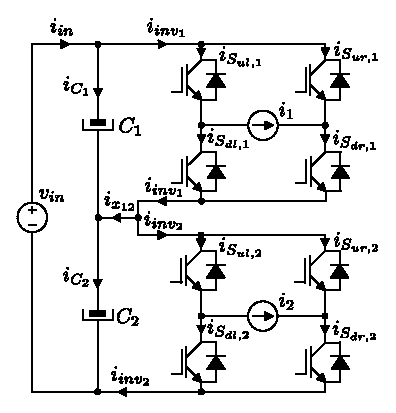
\includegraphics[width=0.75\textwidth]{Figs/MHF1F_ix.eps}
 		\caption{Equivalent circuit used to analyze the capacitor voltage for two sub-modules.}
 		\label{fig:MHF1F_ix}
 	\end{minipage}
 	\quad
 	\begin{minipage}[b]{0.45\textwidth} 	\centering
 		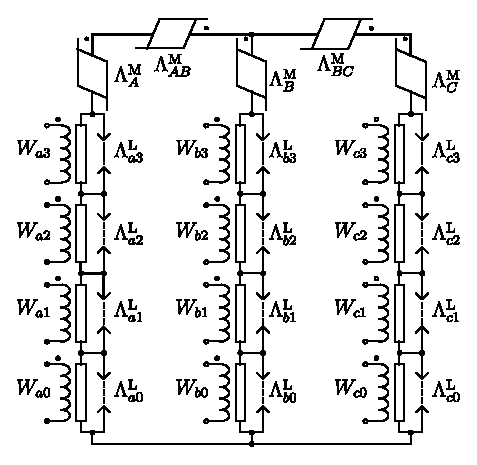
\includegraphics[width=0.8\linewidth]{Figs/MagneticCircuit}
 		\caption{Magnetic circuit implemented in the software PSIM.}
 		\label{fig:MagneticCircuit}
 	\end{minipage}
 \end{figure}
 

\begin{minipage}[b]{0.55\textwidth}
	 \begin{eqnarray}
         {v_{ds}} &=& {R_s}{i_{ds}} + \frac{{d{\psi _{ds}}}}{{dt}} - {\omega _a}{\psi _{qs}}\\
         {v_{qs}} &=& {R_s}{i_{qs}} + \frac{{d{\psi _{qs}}}}{{dt}} - {\omega _a}{\psi _{ds}}\\
         {v_{dr}} = 0 &=& {R_r}{i_{qs}} + \frac{{d{\psi _{dr}}}}{{dt}} - \left( {{\omega _a} - \omega } \right){\psi _{qr}}\\
         {v_{qr}} = 0 &= &{R_r}{i_{qr}} + \frac{{d{\psi _{qr}}}}{{dt}} - \left( {{\omega _a} - \omega } \right){\psi _{dr}}
 \end{eqnarray}
\end{minipage}
\quad
\begin{minipage}[b]{0.35\textwidth} 
	 \begin{eqnarray}
	{v_{xks}} &=& {R_s}{i_{xks}} + \frac{{d{\psi _{xks}}}}{{dt}}\\
	{v_{yks}} &=& {R_s}{i_{yks}} + \frac{{d{\psi _{yks}}}}{{dt}}\\	
	{v_{0s}} &=& {R_s}{i_{0s}} + \frac{{d{\psi _{0s}}}}{{dt}}\\
	{\psi _{0s}} &=& {L_{ls}}{i_{0s}}
	\end{eqnarray}
\end{minipage}    		

  	
  	
 
 
 
 
 
 
 
 

  \subsection{Tables}
 
 
 \begin{table}[ht]
 	\centering
 	\begin{minipage}[b]{0.45\textwidth}	
 		\caption{Prototype Values.}
 		\label{tab:PrototypeDetails}
 		\centering
 		\resizebox{\textwidth}{!}{%
 			\begin{tabular}{c|c|c} \toprule
 				\textbf{Parameter}& \textbf{Value} & \textbf{Description} \\ \midrule
 				$P_{k}$ & 2 kW & Output rated power per sub--module\\
 				$V_k$ & 220 V & Output rated voltage per sub--module\\
 				$V_{in}$   & 1200 V & Input dc bus voltage  \\ 
 				$f_s$   & 19980 Hz & Switching frequency \\ 
 				$f_o$   & 60 Hz & Fundamental frequency\\ 
 				$C_k$   & 1020 $\mu$F & Bus capacitor capacitance \\ 
 				$L_k$   & 1 mH & Filtering inductance \\
 				$n_k$   & 1:1:1:1 & Transformer transformation ratio per phase  \\ 
 				$k$& 3& Number of inverters per phase (sub--modules) \\ 
 				$R_0$   & 8 $\Omega$ & Load resistance \\ 
 				$C_0$   & 15 $\mu$F & Load capacitance \\ 
 				$L_0$   & 5 mH & Load inductance \\
 				\bottomrule
 			\end{tabular}}
 		\end{minipage}
 		\quad
 		\begin{minipage}[b]{0.45\textwidth} 
 			\caption{Simulation RMS values with applied parameters.}
 			\label{tab:SimulationResults}
 			\centering
 			\resizebox{\textwidth}{!}{%
 				\begin{tabular}{cc|cc|cc} \toprule 
 					\multicolumn{2}{l}{\textbf{Phase A} } & \multicolumn{2}{l}{\textbf{Phase B}} 
 					& \multicolumn{2}{l}{\textbf{Phase C}} \\ \hline
 					Parameter       & Value       & Parameter        & Value        & Parameter         & Value            \\\hline
 					$I_{La1}$&$\SI{9.0145887e+000}{\A}$&  $I_{Lb1}$&$\SI{9.9448656e+000}{\A}$& $I_{Lc1}$&$\SI{9.1877882e+000}{\A}$ \\
 					$I_{La2}$&$\SI{8.9496558e+000}{\A}$&  $I_{Lb2}$&$\SI{9.8979341e+000}{\A}$& $I_{Lc2}$&$\SI{9.0625976e+000}{\A}$ \\
 					$I_{La3}$&$\SI{8.9564445e+000}{\A}$&  $I_{Lb3}$&$\SI{9.8901011e+000}{\A}$& $I_{Lc3}$&$\SI{9.0550971e+000}{\A}$ \\
 					$P_{a1}$& $\SI{2017.5626e+000}{\W}$&  $P_{b1}$& $\SI{2200.6884e+000}{\W}$& $P_{c1}$& $\SI{2017.7425e+000}{\W}$ \\
 					$P_{a2}$& $\SI{2015.9731e+000}{\W}$&  $P_{b2}$& $\SI{2199.8454e+000}{\W}$& $P_{c2}$& $\SI{2014.4103e+000}{\W}$ \\
 					$P_{a3}$& $\SI{2015.8540e+000}{\W}$&  $P_{b3}$& $\SI{2199.2212e+000}{\W}$& $P_{c3}$& $\SI{2013.9296e+000}{\W}$ \\
 					$Q_{a1}$& $\SI{524.74548e+000}{\VA}$&  $Q_{b1}$& $\SI{615.93981e+000}{\VA}$& $Q_{c1}$& $\SI{679.69434e+000}{\VA}$ \\
 					$Q_{a2}$& $\SI{452.40163e+000}{\VA}$&  $Q_{b2}$& $\SI{579.60158e+000}{\VA}$& $Q_{c2}$& $\SI{573.18841e+000}{\VA}$ \\
 					$Q_{a3}$& $\SI{458.56979e+000}{\VA}$&  $Q_{b3}$& $\SI{568.68134e+000}{\VA}$& $Q_{c3}$& $\SI{562.90249e+000}{\VA}$ \\
 					$V_{Ca1}$&$\SI{400.30184e+000}{\V}$&  $V_{Cb1}$&$\SI{400.21506e+000}{\V}$& $V_{Cc1}$&$\SI{400.56338e+000}{\V}$ \\
 					$V_{Ca2}$&$\SI{399.83914e+000}{\V}$&  $V_{Cb2}$&$\SI{400.04345e+000}{\V}$& $V_{Cc2}$&$\SI{399.84252e+000}{\V}$ \\
 					$V_{Ca3}$&$\SI{399.85999e+000}{\V}$&  $V_{Cb3}$&$\SI{399.74261e+000}{\V}$& $V_{Cc3}$&$\SI{399.59499e+000}{\V}$ \\
 					$I_{Ca1}$&$\SI{3.5236129e+000}{\A}$&  $I_{Cb1}$&$\SI{3.8862845e+000}{\A}$& $I_{Cc1}$&$\SI{3.5822843e+000}{\A}$ \\
 					$I_{Ca2}$&$\SI{3.5151951e+000}{\A}$&  $I_{Cb2}$&$\SI{3.8834127e+000}{\A}$& $I_{Cc2}$&$\SI{3.5612719e+000}{\A}$ \\
 					$I_{Ca3}$&$\SI{3.5107804e+000}{\A}$&  $I_{Cb3}$&$\SI{3.8751641e+000}{\A}$& $I_{Cc3}$&$\SI{3.5525851e+000}{\A}$ \\
 					\bottomrule                                                                                          
 				\end{tabular}}
 			\end{minipage}
 		\end{table}
 		
 		
 		

\section{CONCLUSION}
A conclusion might elaborate on the importance of the work or suggest
applications and extensions. Clearly indicate advantages, limitations and
possible applications.

%\section*{ACKNOWLEDGEMENT}
%A brief acknowledgement section may be included here.
 		
 
% trigger a \newpage just before the given reference
% number - used to balance the columns on the last page
% adjust value as needed - may need to be readjusted if
% the document is modified later
%\IEEEtriggeratref{8}
% The "triggered" command can be changed if desired:
%\IEEEtriggercmd{\enlargethispage{-5in}}

% references section

% can use a bibliography generated by BibTeX as a .bbl file
% BibTeX documentation can be easily obtained at:
% http://www.ctan.org/tex-archive/biblio/bibtex/contrib/doc/
% The IEEEtran BibTeX style support page is at:
% http://www.michaelshell.org/tex/ieeetran/bibtex/


\bibliographystyle{IEEEtran}
% argument is your BibTeX string definitions and bibliography database(s)
\bibliography{IEEEabrv,IEEEexample}
%
% <OR> manually copy in the resultant .bbl file
% set second argument of \begin to the number of references
% (used to reserve space for the reference number labels box)
%\begin{thebibliography}{1}
%
%\bibitem{IEEEhowto:kopka}
%H.~Kopka and P.~W. Daly, \emph{A Guide to \LaTeX}, 3rd~ed.\hskip 1em plus
%  0.5em minus 0.4em\relax Harlow, England: Addison-Wesley, 1999.
%
%\end{thebibliography}




% that's all folks
\end{document}


